% ------------------------------------------------------------------------------
% TYPO3 CMS 8 LTS - What's New - Chapter "Backend User Interface" (English Version)
%
% @author	Michael Schams <schams.net>
% @license	Creative Commons BY-NC-SA 3.0
% @link		http://typo3.org/download/release-notes/whats-new/
% @language	English
% ------------------------------------------------------------------------------
% LTXE-CHAPTER-UID:		a4c76099-c7aef102-9c114217-0e87f17d
% LTXE-CHAPTER-NAME:	CKEditor
% ------------------------------------------------------------------------------

\section{Rich Text Editor}
\begin{frame}[fragile]
	\frametitle{Rich Text Editor}

	\begin{center}\huge{\color{typo3darkgrey}\textbf{Rich Text Editor}}\end{center}
	\begin{center}\large{\textit{Content editing taken a huge step further}}\end{center}

\end{frame}

% ------------------------------------------------------------------------------
% LTXE-SLIDE-START
% LTXE-SLIDE-UID:		9d35effa-86de2791-6e57298b-bf673c19
% LTXE-SLIDE-TITLE:		CKEditor: Quick Facts
% ------------------------------------------------------------------------------
\begin{frame}[fragile]
	\frametitle{Rich Text Editor}
	\framesubtitle{CKEditor Integration}

	\begin{itemize}

		\item New Rich Text Editor (RTE) was implemented: \textbf{CKEditor}
		\item Well-known and widely used in the PHP universe, easy to configure
		\item Replaces "HtmlArea" and lays the foundation for frontend editing in the near future
		\item HtmlArea is still available as an optional extension in the TYPO3 Extension Repository (TER)

		\item Crowdfunding campaign initiated by the Swedish web agency
			\href{http://pixelant.net}{Pixelant AB} raised more than
			63,000.- Euro (110+ supports worldwide)

	\end{itemize}

\end{frame}

% ------------------------------------------------------------------------------
% LTXE-SLIDE-START
% LTXE-SLIDE-UID:		e99e7216-970412d5-5614a450-364ddba8
% LTXE-SLIDE-TITLE:		CKEditor Integration
% ------------------------------------------------------------------------------
\begin{frame}[fragile]
	\frametitle{Rich Text Editor}
	\framesubtitle{Screenshots}

	\begin{columns}[T]
		\begin{column}{.5\textwidth}
			\begin{figure}\vspace*{-0.4cm}
				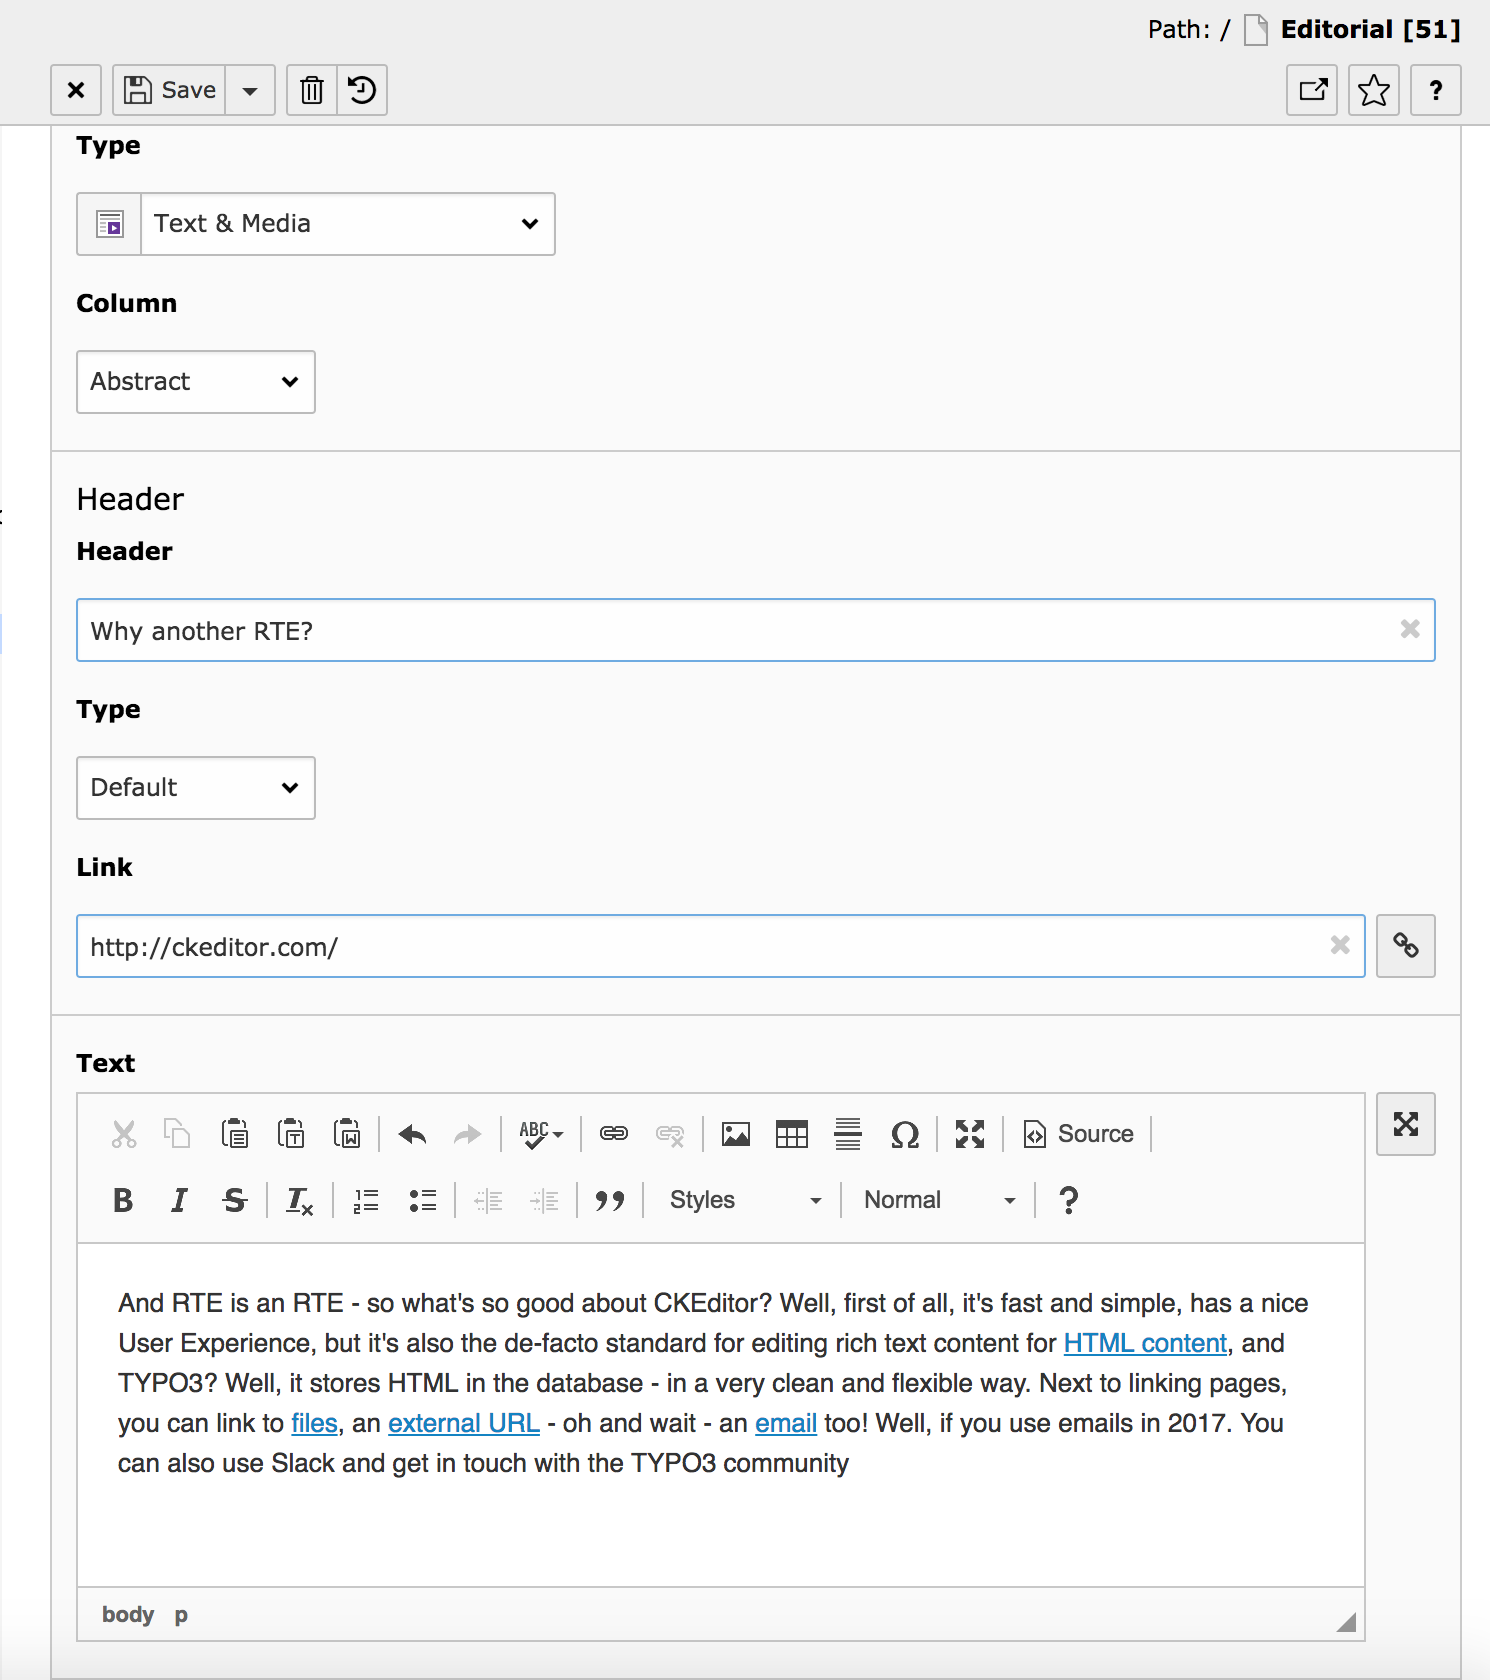
\includegraphics[width=0.8\linewidth]{CKEditor/ckeditor-1.png}
			\end{figure}
		\end{column}
		\begin{column}{.5\textwidth}
%			\begin{figure}\vspace*{-0.4cm}
%				
\includegraphics[width=0.8\linewidth]{CKEditor/ckeditor-2.png}
%			\end{figure}
		\end{column}
	\end{columns}

\end{frame}

% ------------------------------------------------------------------------------
